\documentclass{article}

\usepackage{geometry}
\usepackage{hyperref}
\usepackage{graphicx}
\usepackage{float}
\usepackage{cite}
\title {CS 201: Data Structures II \\Merkle Trees} % Mention your project title

\author{L5- Group 2} % Mention your team name
\date{Spring 2023}  

\begin{document}
\maketitle
\section{Group Members}
% Mention your Group Members and their ids
\begin{enumerate}
  \item Muzzammil Sattar ms07164
  \item Arsalan Hussain mh07607
  \item Abdullah Junejo aj07154
  \item Anas Bin Yousuf ab07351
\end{enumerate}
\section{Data Structure}
We will create a localized implementation of block-chain using Merkle trees and a simple Linked List. 
Merkle trees will be used to encrypt the data using a collision resistant hash function. 
\section{Application}
We will demonstrate encryption and security of documents by using our own block chain. We will further show how a Merkle Tree effectively identifies if any given document has been changed or corrupted.  
\section{Functionality}
We will use two data structures to simulate a blockchain:
\subsection{Linked List}
The Linked List will consist of blocks. Each block will have its own ID, contain the files associated with the block, the root hash of its Merkle 
tree, and hash of the previous block. In this way, multiple blocks 
will be chained to form a block chain. The Linked List interface will consist of three main functionalities:
\begin{enumerate}
\item add: The add function will take in input the list of files and create a block using that list and add it to the blockchain by setting its previous hash to the hash of head of the blockchain. 
\item verify: The verify function is responsible for verifying the integrity of the chain. This involves traversing the chain from the most recent block back to the genesis block (first block created), verifying each block's hash against the hash of the previous block. If any block's hash is found to be incorrect, it indicates that the chain has been tampered with and is no longer valid. If all blocks' hashes are correct, it indicates that the chain is valid and has not been tampered with. 
\\\\ We may use an alternate and more robust implementation of verify function which will 
be able to check for tampering even when the program isn't running by storing the hash value(s) of the blockchain
in a csv file and then comparing the current hash values with those stored values in the csv files. 
\item read: The read function will be passed a block ID, it will then traverse through the blockchain and find the block with the given ID. Then it will print all the data in all of the documents containted within that block. 
\end{enumerate}
\subsection{Merkle Tree}
The Merkle Tree has two key functions: 
\\\\
1) Encryption: This is where the Merkle Tree (or Block) is created using the decided data/documents and collision resistant hash function.
\\\\
2) Verification: This is where we use Merkle Proofs to efficiently check if a given data/document belongs to the Tree and also to verify (through hashing) if the given data/document has been altered or corrupted.
\\\\
We will now talk about Encryption and the creation of the Merkle Tree in a little more depth:
\\\\
To construct the Merkle Tree we start at the leaf nodes, and create layers until we reach the root node which is our root hash. 
\\\\
For example if we have 8 documents we will hash all 8 documents to produce 8 hashes, this is our zeorth layer. We will then hash each pair (Document 1's hash with Document 2's, Document 3's hash with Document 4's, Document 5's hash with Document 6's). This will result in 4 hashes that make up the first layer. Pairs of these four hashes are then hashed together to form the second layer consisting of two hashes, which are then hashes together to form the root hash. The image below illustrates this:

\begin{figure}[htp]
    \centering
    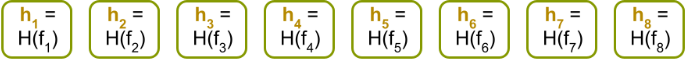
\includegraphics[width=12cm]{Layer 0}
    \caption{The Zeroth Layer}
    \label{fig:f1}
\end{figure}

\begin{figure}[htp]
    \centering
    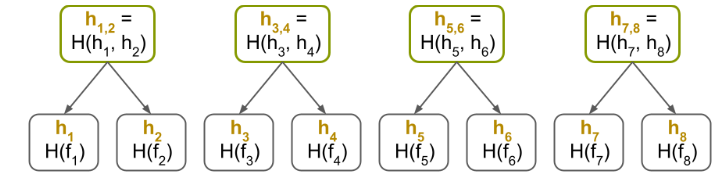
\includegraphics[width=12cm]{Layer 1}
    \caption{The First Layer}
    \label{fig:f2}
\end{figure}

\begin{figure}[htp]
    \centering
    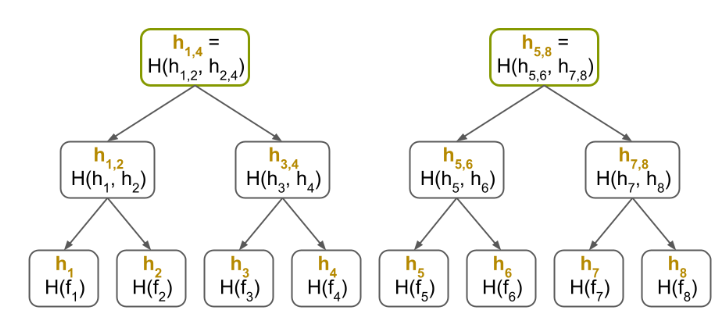
\includegraphics[width=12cm]{Layer 2}
    \caption{The Second Layer}
    \label{fig:f3}
\end{figure}

\begin{figure}[htp]
    \centering
    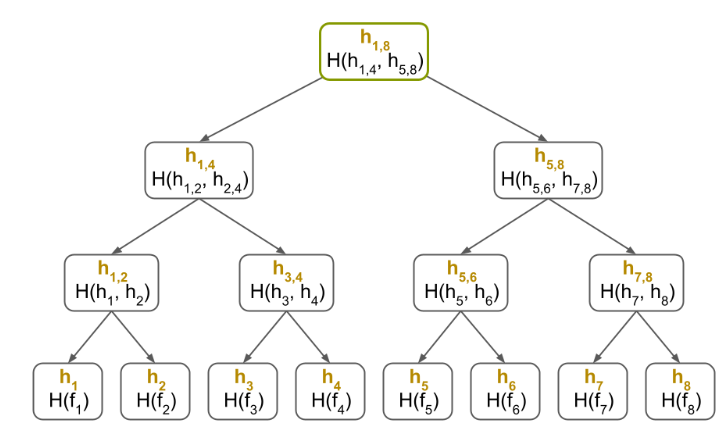
\includegraphics[width=12cm]{Final Layer}
    \caption{The Final Layer and Root Hash}
    \label{fig:f4}
\end{figure}

.
\\\\\\
This can be done for any n number of documents, where after the zeroth layer we hash the pairs to produce n/2 hashes. Those pairs are then hashed to produce n/4 hashes and so on until we reach n/n hashes which is the final layer that is the root hash.
\\\\
Once a Merkle Tree or Block has been created no other documents can be added to it. If there is a new related set of documents that need to be inserted, these documents are made into their own Merkle Tree or Block. The Blocks are then linked together using a simple Link List.
\\\\
We will now discuss the verification process:
\\\\
Merkle Tree's are efficient at verifying if a document has been changed as an altered document would produce a hash that is different from the root hash. If the document hasn't been changed then the same root hash would be produced. This is the bases of a Merkle Proof. Furthermore only a set of hashes would be needed to prove a given leaf's membership in the tree as illustrated below for the example discussed earlier:

\begin{figure}[htp]
    \centering
    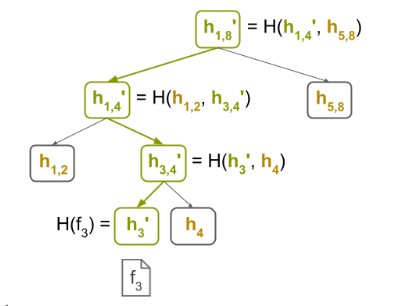
\includegraphics[width=8cm]{Merkle Proof}
    \caption{Merkle Proof}
    \label{fig:f4}
\end{figure}
.
\\\\\\\\\\
\section{Datasets}
It will be fitting to use a part of Bitcoin historical dataset like this \href{https://www.kaggle.com/datasets/prasoonkottarathil/btcinusd}{ one}. We want to take multiple csv files as input to make multiple blocks and then try edititng the csv files to check for the Validation Functionality. However, we are not completely sure about the feasibility of using such a huge dataset. It should be noted that our dataset is one which we should be able to change or corrupt after using it to make the Merkle Tree to demonstrate its Validation Functionality. 

\newpage
\section{Work Distribution}
Fill in the table which indicates the work distribution of each member.
\begin{center}
  \begin{table}[h]
    \centering
    \begin{tabular}{|c|c|c|}
      \hline
      Item & Activity   & ID      \\ \hline
      
      1    & Validating Blockchain and verifying existence of node in Merkle Tree (Merkle Proof)   & mh07607 \\ \hline
      2    & Generating Blockchain on data input (Encrypting and Securing the Data) & ms07164 \\ \hline
      3    & Implementing Blockchain interface and retrieving/storing data from dataset & ab07351 \\ \hline
      4    & Merkle Tree implementation and storing block information on csv file & aj07154 \\ \hline
    \end{tabular}

    \label{tab:my-table6}
  \end{table}
\end{center}
\section{Attribution}

\begin{thebibliography}{9}
  \bibitem{decentralizedthoughts}
Decentralized Thoughts. (2020, December 22). \textit{What is a Merkle Tree?} Retrieved April 4, 2023, from \url{https://decentralizedthoughts.github.io/2020-12-22-what-is-a-merkle-tree/}
  \bibitem{geeksforgeeks}
GeeksforGeeks. (2018). \textit{Introduction to Merkle Tree}. Retrieved April 4, 2023, from \url{https://www.geeksforgeeks.org/introduction-to-merkle-tree/}

  \end{thebibliography}
\end{document}

